\documentclass{beamer}
\usetheme{Rochester}
\setbeamertemplate{navigation symbols}{}

\usepackage{seraf}
\usepackage{url}
\usepackage{graphicx}
\usepackage{tikz}
\usepackage{pgfplots}

\usepackage{isabelle, isabellesym}

\newcommand\var{\mathop{\text{var}}}
\newcommand\bldseq[2]{\langle{#1}\mid{#2}\rangle}
\newcommand\Si{\text{Si}}
\newcommand\bldset[2]{\{{#1}\mid{#2}\}}

\title{A Formally Verified Proof of the \protect\\ Central Limit Theorem}
\author{Luke Serafin}
\institute{Carnegie Mellon University}
\date{\today}

\begin{document}

\begin{frame}
\titlepage
\end{frame}

\begin{frame}
\tableofcontents
\end{frame}

\section{Introduction}

\begin{frame}
\frametitle{A Repeated Coin Toss}
\begin{center}
\begin{tikzpicture}
  \begin{axis}[width=10cm, height=5cm,
      xmin = -5,
      xmax = 5,
      ymin = 0,
      ymax = 0.5,
      ytick = \empty,
      ybar, bar shift = {0cm},
      bar width = 2pt]
    
    \only<4>{\addplot[fill=red!30] table {binomial-128.dat};}
    \only<3>{\addplot[fill=red!50] table {binomial-32.dat};}
    \only<2>{\addplot[fill=red!70] table {binomial-8.dat};}
    \only<1>{
      \addplot[fill=red!90] table {binomial-2.dat};
    }
  \end{axis}
\end{tikzpicture}
\end{center}

\begin{center}
\only<1>{$n = 4$} \only<2>{$n = 16$} \only<3>{$n = 64$} \only<4>{$n = 256$}
\end{center}
\end{frame}

\begin{frame}
\frametitle{Galton on the Central Limit Theorem}
Sir Francis Galton gave the following poetic characterization of the central limit theorem in 1889: \pause

\begin{quote}
 I know of scarcely anything so apt to impress the imagination as the wonderful form of cosmic order expressed by the ``Law of Frequency of Error.'' The law would have been personified by the Greeks and deified, if they had known of it. It reigns with serenity and in complete self-effacement, amidst the wildest confusion. The huger the mob, and the greater the apparent anarchy, the more perfect is its sway. It is the supreme law of Unreason. Whenever a large sample of chaotic elements are taken in hand and marshaled in the order of their magnitude, an unsuspected and most beautiful form of regularity proves to have been latent all along.
\end{quote}
\end{frame}

\begin{frame}
\frametitle{Galton's Illustration of the Central Limit Theorem}
Galton also invented a device for illustrating the central limit theorem, called variously a Galton box, Galton machine, bean machine, or quincunx. \pause

\center{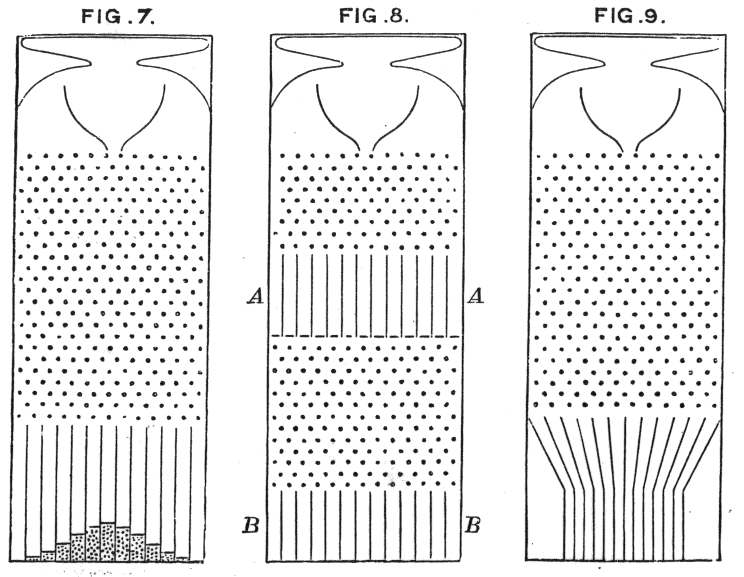
\includegraphics[scale=0.25]{Galton_machine_diagram.png}}
\end{frame}

\begin{frame}
\frametitle{A Galton Machine}
\url{https://www.youtube.com/watch?v=9xUBhhM4vbM}
\end{frame}

\begin{frame}
\frametitle{The Normal Distribution}
Let $B$ be a Borel subset of $\R$.
\[ \mathcal N_{0,1}(B) = \frac{1}{\sqrt {2\pi}} \int_B e^{-x^2/2} \, dx \] \pause
\center{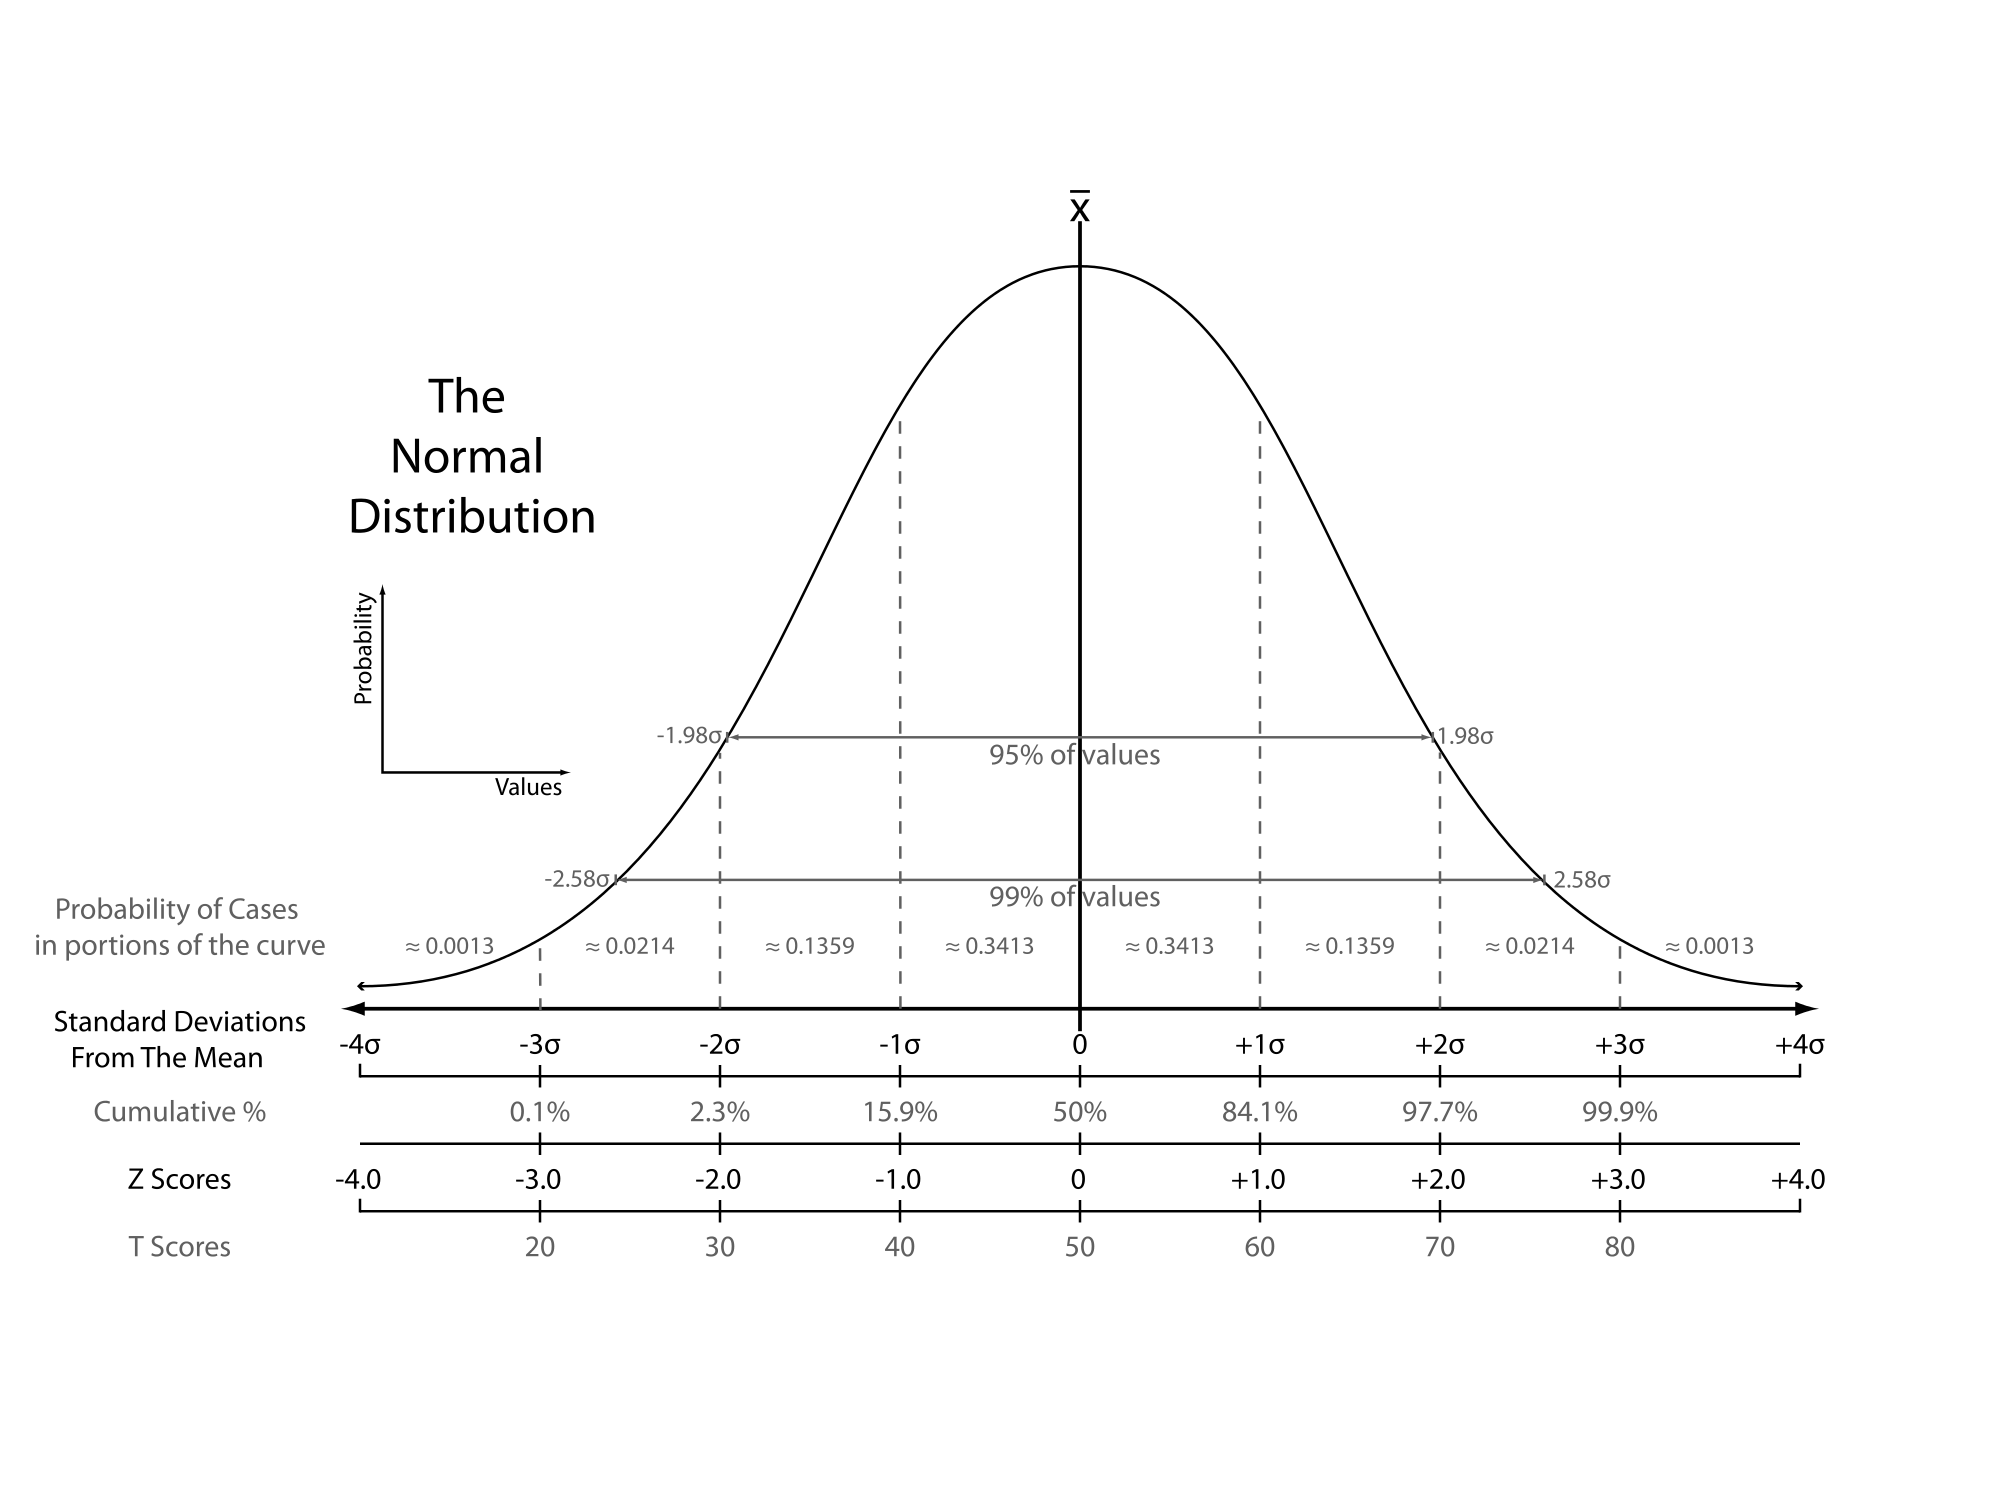
\includegraphics[scale=0.13]{Normal_Distribution.png}}
\end{frame}

\begin{frame}
\frametitle{Informal Statement of the Central Limit Theorem}
If an experiment with a random, numeric outcome with finite, nonzero variance is carried out repeatedly, the average value of the outcomes observed approaches a normal distribution.
\end{frame}

\begin{frame}
\frametitle{Statement of the Central Limit Theorem}
Let $\bldseq{X_n}{n \in \N}$ be independent, identically distributed random variables with finite, nonzero variance. \pause

Assume without loss of generality that
\[ \E(X_n) = 0, \var(X_n) = \E((X_n - \E(X_n))^2) = 1. \] \pause

The central limit theorem states that
\[ \lim_{n \rightarrow \infty} \frac{1}{n}\sum_{k \le n} X_k \Rightarrow \mathcal N_{0,1}. \]
\end{frame}

\section{Outline of Proof}

\begin{frame}
\frametitle{Convergence in Distribution}
The right notion of convergence for the central limit theorem is known as convergence in distribution (or weak convergence). \pause
\begin{definition}
Let $\bldseq{\mu_n}{n \in \N}$ be a sequence of Borel probability measures on $\R$. This sequence converges {\em in distribution} (or {\em weakly}) to a probability measure $\mu$, denoted $\mu_n \Rightarrow \mu$, iff for every $x \in \R$ such that $\mu \{x\} = 0$, $\mu_n (-\infty, x] \rightarrow \mu (-\infty, x]$.
\end{definition}
\end{frame}

\begin{frame}
\frametitle{Characteristic Functions}
To study convergence in distribution, it turns out to be most convenient to take Fourier transforms, which are called characteristic functions in a probabilistic context. \pause

\begin{definition}
Let $\mu$ be a Borel probability measure on $\R$. The {\em characteristic function} of $\mu$ is the function $\phi\colon \R \rightarrow \C$ given by
\[ \phi(x) = \int e^{itx} \, \mu(dt). \]
\end{definition}
\end{frame}

\begin{frame}
\frametitle{The L\'evy Continuity Theorem}
An important reason for passing to characteristic functions is the L\'evy continuity theorem, which allows one to replace the analytically complicated notion of convergence in distribution with the much simpler notion of pointwise convergence. \pause

\begin{theorem}
Let $\bldseq{\mu_n}{n \in \N}$, $\mu$ be Borel probability measures on $\R$, and $\bldseq{\phi_n}{n \in \N}$, $\phi$ be their corresponding characteristic functions. Then $\mu_n \Rightarrow \mu$ iff $\phi_n \rightarrow \phi$ pointwise.
\end{theorem}
\end{frame}

\begin{frame}
In order to exploit the L\'evy continuity theorem, we need the fact that characteristic functions uniquely characterize their distributions, which follows from the L\'evy inversion theorem. \pause

\begin{theorem}
Let $\mu$ be a probability measure, and $\phi$ be the characteristic function of $\mu$. If $\mu \{a\} = \mu \{b\} = 0$ and $a < b$, then
\[ \mu (a,b] = \lim_{T \rightarrow \infty} \frac{1}{2\pi} \int_{-T}^T \frac{e^{-ita} - e^{-itb}}{it} \phi(t) \, dt. \]
Hence distinct probability measures have distinct characteristic functions.
\end{theorem}
\end{frame}

\begin{frame}
\frametitle{Convolutions}
If $X$ and $Y$ are independent random variables and $X \sim \mu$, $Y \sim \nu$, then the distribution of $X + Y$ is the convolution $\mu * \nu$, which is defined by
\[ (\mu * \nu)(B) = \int \nu(B - x) \mu(dx), \]
where $B$ is any Borel subset of $\R$ and $B - x = \bldset{y - x}{y \in B}$.
\end{frame}

\begin{frame}
\frametitle{Convolutions and Characteristic Functions}
Another good reason for using characteristic functions in the proof of the central limit theorem is the fact that they greatly simplify working with convolutions. \pause

\begin{lemma}
If $\mu$, $\nu$ are Borel probability measures on $\R$ with characteristic functions $\phi$ and $\psi$, respectively, then the characteristic function of $\mu * \nu$ is the pointwise product $\phi\psi$.
\end{lemma}
\end{frame}

\begin{frame}
\frametitle{$n$-fold Convolutions}
The average $n\inv \sum_{k \le n} X_k$ in the statement of the central limit theorem is distributed as a multiple of the $n$-fold convolution of $X_1$ with itself (recall that the $X_k$'s are identically distributed). \pause Working with this is greatly simplified by passing to characteristic functions, because the $n$-fold convolution becomes instead an $n$th power.
\end{frame}

\begin{frame}
\frametitle{Plan of the Proof}
At a high level, the proof of the central limit theorem proceeds by showing that if $\phi$ is the characteristic function of a random variable with zero mean and finite nonzero variance, then
\[ \lim_{n \rightarrow \infty} \phi^n\left(\frac{x}{\sqrt n}\right) = \psi(x), \]
where $\psi$ is the characteristic function of the standard normal distribution $\mathcal N_{0,1}$.
\end{frame}

\section{Interactive Formal Proof-checking in Isabelle}

\begin{frame}
\frametitle{Formal Proofs}
\begin{itemize}
\item Significant developments in logic in the 19th and 20th centuries allowed the notion proof to be formalized with mathematical rigour. \pause
\item However, writing proofs is in general impractical for human mathematicians. \pause
\item Developments in computing technology have allowed computers to verify many tedious formal details automatically. \pause
\item Interactive theorem proving consists in a human specifying a high-level outline of a proof, which is then checked in full formal detail by a computer.
\end{itemize}
\end{frame}

\begin{frame}
\frametitle{Previous Formalization}
\begin{itemize}
\item Several significant mathematical results already formally verified. \pause
\item Prime number theorem an early result, with effort lead by Avigad. \pause
\item Often elementary proofs are chosen to facilitate formalization (as in case of prime number theorem).
\end{itemize}
\end{frame}

\begin{frame}
\frametitle{Motivation for the CLT}
\begin{itemize}
\item We wanted to improve the integration libraries of Isabelle. \pause
\item Avigad suggested choosing a specific result to work toward. \pause
\item We chose the central limit theorem as a significant result with a deep analytic proof.
\end{itemize}
\end{frame}

\begin{frame}
\frametitle{Isabelle Overview}
Isabelle is a general-purpose interactive proof assistant initially developed by Larry Paulson at Cambridge University and Tobias Nipkow at Technische Universit\"at M\"unchen.
\end{frame}

\begin{frame}
\frametitle{Isabelle Overview}
\begin{itemize}
\item Isabelle supports reasoning in a wide variety of logics. \pause
\item We worked with Isabelle/HOL. \pause
\item Background logic extension of higher-order logic. \pause
\item Adds inductively defined types (e.g. natural numbers) and an indefinite description operator (which entails the axiom of choice).
\end{itemize}
\end{frame}

\begin{frame}
\frametitle{Interacting with Isabelle}
Full proof scripts available at \url{https://github.com/avigad/isabelle}.
\end{frame}

\begin{frame}
\frametitle{Analysis in Isabelle}
\begin{itemize}
\item Filterlimit and measure theory libraries developed by Johannes H\"olzl at Technische Universit\"at M\"unchen. \pause
\item $\pi$-$\lambda$ theorem. \pause
\item Carath\'eodory extension theorem. \pause
\item Product measure and Fubini's theorem. \pause
\item Independence of random variables. \pause
\item Much more...
\end{itemize}
\end{frame}

\section{Overview of Formalizations}

\begin{frame}
\frametitle{Formal Statement of the Central Limit Theorem}
\begin{isabellebody}
\isacommand{theorem}\isamarkupfalse%
\ {\isacharparenleft}\,\isakeyword{in}\ prob{\isacharunderscore}space{\isacharparenright}\ central{\isacharunderscore}limit{\isacharunderscore}theorem{\isacharcolon}\isanewline
\ \ \isakeyword{fixes}\ \isanewline
\ \ \ \ X\ {\isacharcolon}{\isacharcolon}\ {\isachardoublequoteopen}nat\ {\isasymRightarrow}\ {\isacharprime}a\ {\isasymRightarrow}\ real{\isachardoublequoteclose}\ \isakeyword{and}\isanewline
\ \ \ \ D\ {\isacharcolon}{\isacharcolon}\ {\isachardoublequoteopen}real\ measure{\isachardoublequoteclose}\ \isakeyword{and}\isanewline
\ \ \ \ {\isasymsigma}\ {\isacharcolon}{\isacharcolon}\ real\isanewline
\pause
\ \ \isakeyword{assumes}\isanewline
\ \ \ \ {\isachardoublequoteopen}indep{\isacharunderscore}vars\ {\isacharparenleft}{\isasymlambda}i{\isachardot}\ borel{\isacharparenright}\ X\ UNIV{\isachardoublequoteclose}\ \isakeyword{and}\isanewline
\ \ \ \ {\isachardoublequoteopen}{\isasymAnd}n{\isachardot}\ {distr}\ M\ borel\ {\isacharparenleft}X\ n{\isacharparenright}\ {\isacharequal}\ D{\isachardoublequoteclose}
\pause\ \isakeyword{and}\isanewline
\ \ \ \ {\isachardoublequoteopen}{\isasymAnd}n{\isachardot}\ integrable\ M\ {\isacharparenleft}X\ n{\isacharparenright}{\isachardoublequoteclose}\ \isakeyword{and}\isanewline
\ \ \ \ {\isachardoublequoteopen}{\isasymAnd}n{\isachardot}\ expectation\ {\isacharparenleft}X\ n{\isacharparenright}\ {\isacharequal}\ {\isadigit{0}}{\isachardoublequoteclose}
\pause\ \isakeyword{and}\isanewline
\ \ \ \ {\isachardoublequoteopen}{\isasymsigma}\ {\isachargreater}\ {\isadigit{0}}{\isachardoublequoteclose}\ \isakeyword{and}\isanewline
\ \ \ \ {\isachardoublequoteopen}{\isasymAnd}n{\isachardot}\ integrable\ M\ {\isacharparenleft}{\isasymlambda}x{\isachardot}\ {\isacharparenleft}X\ n\ x{\isacharparenright}\isactrlsup {\isadigit{2}}{\isacharparenright}{\isachardoublequoteclose}\ \isakeyword{and}\isanewline
\ \ \ \ {\isachardoublequoteopen}{\isasymAnd}n{\isachardot}\ variance\ {\isacharparenleft}X\ n{\isacharparenright}\ {\isacharequal}\ {\isasymsigma}\isactrlsup {\isadigit{2}}{\isachardoublequoteclose}\isanewline
\pause
\ \ \isakeyword{shows}\isanewline
\ \ \ \ {\isachardoublequoteopen}weak{\isacharunderscore}conv{\isacharunderscore}m\ \isanewline
\ \ \ \ \ \ \ \ {\isacharparenleft}{\isasymlambda}n{\isachardot}\ {distr}\ M\ {borel}\ {\isacharparenleft}{\isasymlambda}x{\isachardot}\ {\isasymSum}i{\isacharless}n{\isachardot}\ X\ i\ x\ {\isacharslash}\ sqrt\ {\isacharparenleft}n\ {\isacharasterisk}\ {\isasymsigma}\isactrlsup {\isadigit{2}}{\isacharparenright}{\isacharparenright}{\isacharparenright}\isanewline
\ \ \ \ \ \ \ \ {\isacharparenleft}{density}\ {lborel}\ standard{\isacharunderscore}normal{\isacharunderscore}density{\isacharparenright}{\isachardoublequoteclose}
\end{isabellebody}
\end{frame}

\begin{frame}
\frametitle{Basic Ingredients of the Proof}
\begin{itemize}
\item Definition and basic properties of characteristic functions. \pause
\item L\'evy inversion and continuity theorems. \pause
\item Taylor estimates to demonstrate pointwise convergence of characteristic functions of averages to the characteristic function of $\mathcal N_{0,1}$.
\end{itemize}
\end{frame}

\begin{frame}
\frametitle{Proof of the L\'evy Inversion Theorem}
\begin{itemize}
\item Properties of sine integral function
\[ \Si(t) = \int_0^t \frac{\sin x}{x} \, dx. \] \pause
\item Further estimates and calculations with integrals. \pause
\item Fact that a probability measure has only countably many atoms.
\end{itemize}
\end{frame}

\begin{frame}
\frametitle{Proof of the L\'evy Continuity Theorem}
\begin{itemize}
\item Use other characterizations of weak convergence given by portmanteau theorem. \pause
\item More integral calculations using Fubini's theorem. \pause
\item Exploiting tightness of a sequence of probability measures whose characteristic functions converge pointwise.
\end{itemize}
\end{frame}

\begin{frame}
\frametitle{The Portmanteau Theorem}
The portmanteau theorem is used in the proof of the L\'evy continuity theorem, and shows that convergence in distribution is equivalent to two standard characterizations of weak* convergence in the sense of functional analysis. \pause

\begin{theorem}
Let $\bldseq{\mu_n}{n \in \N}$ be a sequence of measures on $\R$. The following are equivalent:
\begin{enumerate}
\item $\mu_n \Rightarrow \mu$. \pause
\item For each bounded continuous $f\colon \R \rightarrow \R$, $\int f \, d\mu_n \rightarrow \int f \, d\mu$. \pause
\item If $\mu(\partial A) = 0$, then $\mu_n(A) \rightarrow \mu(A)$.
\end{enumerate}
\end{theorem}
\end{frame}

\begin{frame}
\frametitle{Skorohod's Theorem}
The proof of the portmanteau theorem employs Skorohod's theorem, which provides another sense in which convergence in distribution can be replaced by pointwise convergence. \pause

\begin{theorem}
Let $\bldseq{\mu_n}{n \in \N}$, $\mu$ be probability measures on the $\R$, and suppose $\mu_n \Rightarrow \mu$. Then there exists a probability space $(\Omega, \mathcal F, \P)$ and random variables $\bldseq{Y_n}{n \in \N}$, $Y$ on $\Omega$ such that $Y_n \sim \mu_n$ for each $n$, $Y \sim \mu$, and $Y_n \rightarrow Y$ pointwise.
\end{theorem}
\end{frame}

\begin{frame}
\frametitle{Cumulative Distribution Functions}
Skorohod's theorem is proved by reasoning about pseudoinverses of cumulative distribution functions of measures, and we provided the definition and basic properties of these cumulative distribution functions. \pause

\begin{definition}
Let $\mu$ be a Borel probability measure on $\R$. The {\em cumulative distribution function} (or CDF) $F\colon \R \rightarrow \R$ of $\mu$ is given by $F(x) = \mu (-\infty,x]$.
\end{definition}
\end{frame}

\begin{frame}
\frametitle{Basic Properties of CDF's}
Suppose $\mu$ is a Borel probability measure with CDF $F$. \pause
\begin{itemize}
\item $F$ is nondecreasing and right-continuous. \pause
\item $\lim_{x \rightarrow -\infty} F(x) = 0$ and $\lim_{x \rightarrow \infty} F(x) = 1$. \pause
\item The cumulative distribution function uniquely characterizes its distribution.
\end{itemize}
\end{frame}

\begin{frame}
\frametitle{Proof of Skorohod's Theorem}
\begin{theorem}
Let $\bldseq{\mu_n}{n \in \N}$, $\mu$ be probability measures on the $\R$, and suppose $\mu_n \Rightarrow \mu$. Then there exists a probability space $(\Omega, \mathcal F, \P)$ and random variables $\bldseq{Y_n}{n \in \N}$, $Y$ on $\Omega$ such that $Y_n \sim \mu_n$ for each $n$, $Y \sim \mu$, and $Y_n \rightarrow Y$ pointwise.
\end{theorem}

\pause

The random variables $Y_n(\omega)$, $Y(\omega)$ are (almost) given by $\inf \bldset{x}{\omega \le F_n(x)}$ and $\inf \bldset{x}{\omega \le F(x)}$, respectively, these being the pseudoinverses of the distribution functions $F_n$, $F$ of the measures $\mu_n$, $\mu$.
\end{frame}

\begin{frame}
\frametitle{Proof of Skorohod's Theorem}
The remainder of the proof is careful estimation of limits inferior and superior, which show these are close to each other for sufficiently large $n$ away from atoms. \pause

Convergence cannot be guaranteed at atoms, so instead of taking $Y_n$ and $Y$ to be the exactly the psdeudoinverses of the corresponding distribution functions, they are redefined to be zero at atoms. The resulting random variables have the same distributions since the set of atoms has measure zero, as follows from the fact it is countable.
\end{frame}

\begin{frame}
\frametitle{Tightness}
Another ingredient of the proof of the L\'evy continuity theorem is the concept of tightness of sequences of measures, which generalizes boundedness of sequences of real numbers. \pause

\begin{definition}
A sequence $\bldseq{\mu_n}{n \in \N}$ of Borel probability measures is {\em tight} iff for every $\eps > 0$ there exist $a < b$ such that $\mu_n (a,b] \ge 1 - \eps$ for every $n$.
\end{definition}

\pause

If $\mu_n$ is a unit mass at $a_n$, $\bldseq{\mu_n}{n \in \N}$ is tight iff $\bldseq{a_n}{n \in \N}$ is bounded.
\end{frame}

\begin{frame}
\frametitle{Properties of Tightness}
The fact about tightness needed for the proof of the continuity theorem is as follows: \pause

\begin{lemma}
If $\bldseq{\mu_n}{n \in \N}$ is a tight sequence of probability measures such that each subsequence which has a weak limit in fact has the probability measure $\mu$ as its weak limit, then in fact $\mu_n \Rightarrow \mu$.
\end{lemma}

\pause

We derive the lemma as a corollary to this useful characterization of tightness, which is an analogue of the Bolzano-Weierstrass theorem: \pause

\begin{theorem}
A sequence $\bldseq{\mu_n}{n \in \N}$ of probability measures is tight if and only if for every subsequence $\bldseq{\mu_{n_k}}{k \in \N}$ there exists a subsubsequence $\bldseq{\mu_{n_{k_j}}}{j \in \N}$ which converges weakly to some probability measure $\mu$.
\end{theorem}
\end{frame}

\begin{frame}
\frametitle{The Helly Selection Theorem}
The proof of the analogue of Bolzano-Weierstrass for tightness is accomplished by means of the Helly selection theorem, another analogue of the Bolzano-Weierstrass theorem which is of importance also in functional analysis. \pause

\begin{theorem}
Let $\bldseq{F_n}{n \in \N}$ be a sequence of cumulative distribution functions. Then there exists a subsequence $\bldset{F_{n_k}}{n \in \N}$ and a nondecreasing, right continuous function $F$ such that $F_{n_k}(x) \rightarrow F(x)$ provided $F$ is continuous at $x$.
\end{theorem}
\end{frame}

\begin{frame}
\frametitle{Proof of the Helly Selection Theorem}

\begin{itemize}
\item An application of the diagonal method at rationals yields a subsequence $\bldseq{n_k}{n \in \N}$ such that $F_{n_k}(q)$ converges for all $q \in \Q$; the limit is called $G(q)$. \pause
\item Fabian Immler at Technische Universit\"at M\"unchen had already formalized the diagonal method with a view toward formalizing the theory of differential equations. \pause
\item The required limit function is obtained by $F(x) = \inf \bldset{G(q)}{q \in \Q, x < q}$. \pause
\item The remainder of the proof is careful estimation showing the limits superior and inferior become close away from discontinuities of $F$.
\end{itemize}
\end{frame}

\begin{frame}
\frametitle{Proof of the Central Limit Theorem}
The central limit theorem is proved by showing that the characteristic function of the average converges in distribution to the characteristic function of a standard normal distribution. \pause
\end{frame}

\begin{frame}
\frametitle{Formal Statement of the Central Limit Theorem}
\begin{isabellebody}
\isacommand{theorem}\isamarkupfalse%
\ {\isacharparenleft}\,\isakeyword{in}\ prob{\isacharunderscore}space{\isacharparenright}\ central{\isacharunderscore}limit{\isacharunderscore}theorem{\isacharcolon}\isanewline
\ \ \isakeyword{fixes}\ \isanewline
\ \ \ \ X\ {\isacharcolon}{\isacharcolon}\ {\isachardoublequoteopen}nat\ {\isasymRightarrow}\ {\isacharprime}a\ {\isasymRightarrow}\ real{\isachardoublequoteclose}\ \isakeyword{and}\isanewline
\ \ \ \ D\ {\isacharcolon}{\isacharcolon}\ {\isachardoublequoteopen}real\ measure{\isachardoublequoteclose}\ \isakeyword{and}\isanewline
\ \ \ \ {\isasymsigma}\ {\isacharcolon}{\isacharcolon}\ real\isanewline
\ \ \isakeyword{assumes}\isanewline
\ \ \ \ {\isachardoublequoteopen}indep{\isacharunderscore}vars\ {\isacharparenleft}{\isasymlambda}i{\isachardot}\ borel{\isacharparenright}\ X\ UNIV{\isachardoublequoteclose}\ \isakeyword{and}\isanewline
\ \ \ \ {\isachardoublequoteopen}{\isasymAnd}n{\isachardot}\ {distr}\ M\ borel\ {\isacharparenleft}X\ n{\isacharparenright}\ {\isacharequal}\ D{\isachardoublequoteclose}
\ \isakeyword{and}\isanewline
\ \ \ \ {\isachardoublequoteopen}{\isasymAnd}n{\isachardot}\ integrable\ M\ {\isacharparenleft}X\ n{\isacharparenright}{\isachardoublequoteclose}\ \isakeyword{and}\isanewline
\ \ \ \ {\isachardoublequoteopen}{\isasymAnd}n{\isachardot}\ expectation\ {\isacharparenleft}X\ n{\isacharparenright}\ {\isacharequal}\ {\isadigit{0}}{\isachardoublequoteclose}
\ \isakeyword{and}\isanewline
\ \ \ \ {\isachardoublequoteopen}{\isasymsigma}\ {\isachargreater}\ {\isadigit{0}}{\isachardoublequoteclose}\ \isakeyword{and}\isanewline
\ \ \ \ {\isachardoublequoteopen}{\isasymAnd}n{\isachardot}\ integrable\ M\ {\isacharparenleft}{\isasymlambda}x{\isachardot}\ {\isacharparenleft}X\ n\ x{\isacharparenright}\isactrlsup {\isadigit{2}}{\isacharparenright}{\isachardoublequoteclose}\ \isakeyword{and}\isanewline
\ \ \ \ {\isachardoublequoteopen}{\isasymAnd}n{\isachardot}\ variance\ {\isacharparenleft}X\ n{\isacharparenright}\ {\isacharequal}\ {\isasymsigma}\isactrlsup {\isadigit{2}}{\isachardoublequoteclose}\isanewline
\ \ \isakeyword{shows}\isanewline
\ \ \ \ {\isachardoublequoteopen}weak{\isacharunderscore}conv{\isacharunderscore}m\ \isanewline
\ \ \ \ \ \ \ \ {\isacharparenleft}{\isasymlambda}n{\isachardot}\ {distr}\ M\ {borel}\ {\isacharparenleft}{\isasymlambda}x{\isachardot}\ {\isasymSum}i{\isacharless}n{\isachardot}\ X\ i\ x\ {\isacharslash}\ sqrt\ {\isacharparenleft}n\ {\isacharasterisk}\ {\isasymsigma}\isactrlsup {\isadigit{2}}{\isacharparenright}{\isacharparenright}{\isacharparenright}\isanewline
\ \ \ \ \ \ \ \ {\isacharparenleft}{density}\ {lborel}\ standard{\isacharunderscore}normal{\isacharunderscore}density{\isacharparenright}{\isachardoublequoteclose}
\end{isabellebody}
\end{frame}

\section{Conclusions and Future Directions}

\begin{frame}
\frametitle{Effort in Formalization}
\begin{itemize}
\item CLT 4499 lines, or 98 pages. \pause
\item Prime number theorem about 22,300 lines, or 500 pages. \pause
\item Large amounts of library development not included in line count for CLT, but even with these it would be at most 15,000 lines.
\end{itemize}
\end{frame}

\begin{frame}
\frametitle{Library Development}
\begin{itemize}
\item Rewrite of integration library to employ Bochner integration inspired by our formalization of integrals of functions of type $\R \rightarrow \C$. \pause
\item Rewrite guided by lessons learned about integration, such as importance of keeping integration closely tied to integrability. \pause
\item Facts about integration over a set or more specifically an integral imported to library. \pause
\item Various versions of the fundamental theorem of calculus and integration by substitution imported to library.
\end{itemize}
\end{frame}

\begin{frame}
\frametitle{Directions for Future Work}
\begin{itemize}
\item Lindeberg CLT, which replaces requirement that summands be identically distributed with a uniform growth contition normalized by the sum of the variances. \pause
\item Central limit theorem for weakly dependent random variables. \pause
\item Central limit theorem for martingales.
\end{itemize}
\end{frame}

\begin{frame}
\frametitle{Acknowledgements}
\begin{itemize}
\item Thank you to Professor Jeremy Avigad for introducing me to Isabelle, working with me on the formalization of the CLT, and giving me much advice and encouragement. \pause
\item Thank you to Johannes H\"olzl at Technische Universit\"at M\"unchen for taking an interest in our project, for much help with supporting our formalization with Bochner integration and other library items, for cleaning up some of our proofs, and for a great deal of practical advice regarding formalization of probability. \pause
\item Thank you to Professors Sieg and Statman for serving on my master's committee. \pause
\item Thank you to the department of philosophy for supporting me in the summer of 2012 with an LSEC grant. \pause
\item Thank you to the National Science Foundation for supporting me with an REU grant in the summer of 2013.
\end{itemize}
\end{frame}

\begin{frame}[allowframebreaks]
\frametitle{References}
\nocite{*}
\bibliographystyle{amsalpha}
\bibliography{itp}
\end{frame}

\end{document}
